% --- Chapter III: Software Requirement Specification ---
\newpage

\section*{III. Software Requirement Specification}
\addcontentsline{toc}{section}{III. Software Requirement Specification}
\setcounter{section}{3}

% Number subsections in this chapter as 1, 2, ... (consistent with other chapters)
\renewcommand{\thesubsection}{\arabic{subsection}}
\setcounter{subsection}{0}

\subsection{Product Overview}
\label{subsec:product-overview}

\begingroup
\setlength{\parindent}{1.5em}
\setlength{\parskip}{0.8em}

\indent The AI-powered Film Photography Contest Management Platform is a web-based application designed to manage and automate the entire workflow of a film photography competition. The system allows participants to register, submit photographs, and track the status of their submissions. Organizers can create and manage contests, assign judges, review flagged submissions, and publish final results. Judges evaluate photographs based on predefined criteria, while administrators manage user accounts, permissions, and system configurations.

\indent To improve efficiency, fairness, and submission authenticity, the platform integrates an AI Verification Engine to extract EXIF metadata, detect duplicate images, and identify AI-generated content before submissions proceed to the judging stage. A Notification Service delivers important updates, including registration confirmations, submission status, judging progress, and contest results. Overall, the system provides a transparent, secure, and efficient environment for managing film photography competitions.

\endgroup

\begin{figure}[htbp]
    \centering
    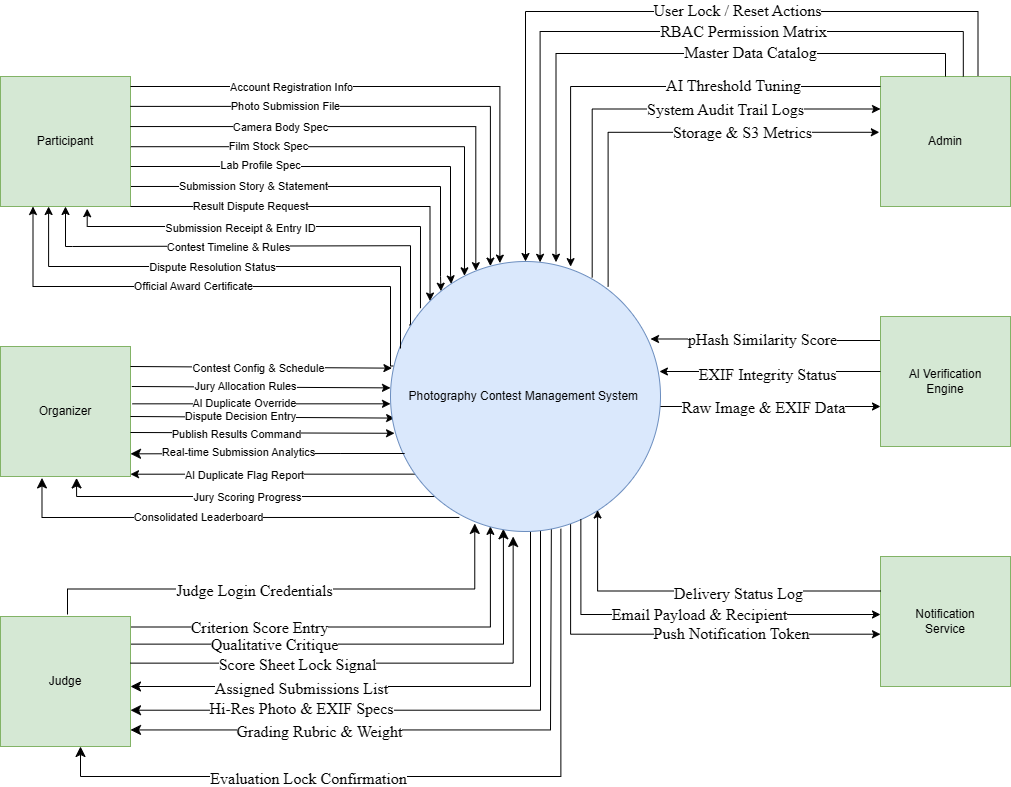
\includegraphics[width=0.95\textwidth]{images/context_diagram}
    \label{fig:context-diagram}
\end{figure}

\subsection{User Requirements}
\label{subsec:user-requirements}

\setcounter{secnumdepth}{4}
\setcounter{tocdepth}{4}
\renewcommand{\theparagraph}{\thesubsubsection.\arabic{paragraph}}

\subsubsection{System Actors}
\label{subsubsec:system-actors}

\renewcommand{\arraystretch}{1.15}
\setlength{\tabcolsep}{6pt}
\begin{longtable}{|>{\centering\arraybackslash}p{0.06\textwidth}|>{\raggedright\arraybackslash}p{0.28\textwidth}|>{\raggedright\arraybackslash}p{0.60\textwidth}|}
\hline
\multicolumn{1}{|c|}{\textbf{No.}} & \multicolumn{1}{c|}{\textbf{Actor}} & \multicolumn{1}{c|}{\textbf{Description}} \\
\hline
\endfirsthead
\multicolumn{1}{|c|}{\textbf{No.}} & \multicolumn{1}{c|}{\textbf{Actor}} & \multicolumn{1}{c|}{\textbf{Description}} \\
\hline
\endhead
\hline
\endfoot
\hline
\endlastfoot
1 & Administrator & Responsible for overall system configuration, managing user accounts, enforcing RBAC (Role-Based Access Control) permissions, tuning AI detection thresholds, managing camera/film master data catalogs, and monitoring system audit trail logs. \\
\hline
2 & Organizer & A contest management authority responsible for setting up competitions, configuring evaluation rubrics, allocating judges, reviewing AI duplicate/fraud flags, handling dispute entries, and publishing final competition results. \\
\hline
3 & Judge & A designated evaluator responsible for logging in, viewing assigned submission queues, evaluating submissions against multi-criteria rubrics, providing qualitative feedback, and locking score sheets. \\
\hline
4 & Participant & A registered user (candidate) who uses the system to browse contests, submit photo entries along with camera/film metadata, track submission status, receive evaluation feedback, and submit result dispute requests. \\
\hline
5 & AI Verification Engine (System Actor) & An external automated service that processes uploaded raw images and EXIF data to compute pHash similarity scores, detect potential duplicate submissions, and flag AI-generated or manipulated images. \\
\hline
6 & Notification Service (System Actor) & An external communication provider responsible for delivering transaction emails, submission receipts, evaluation status updates, and system push notifications to participants and staff. \\
\hline
\end{longtable}

\subsubsection{Use Cases}
\label{subsubsec:use-cases}

\paragraph*{2.2.1 Use Case Diagram}
\label{par:use-case-diagram}
\addcontentsline{toc}{paragraph}{\protect\numberline{2.2.1}Use Case Diagram}

\begin{figure}[htbp]
    \centering
    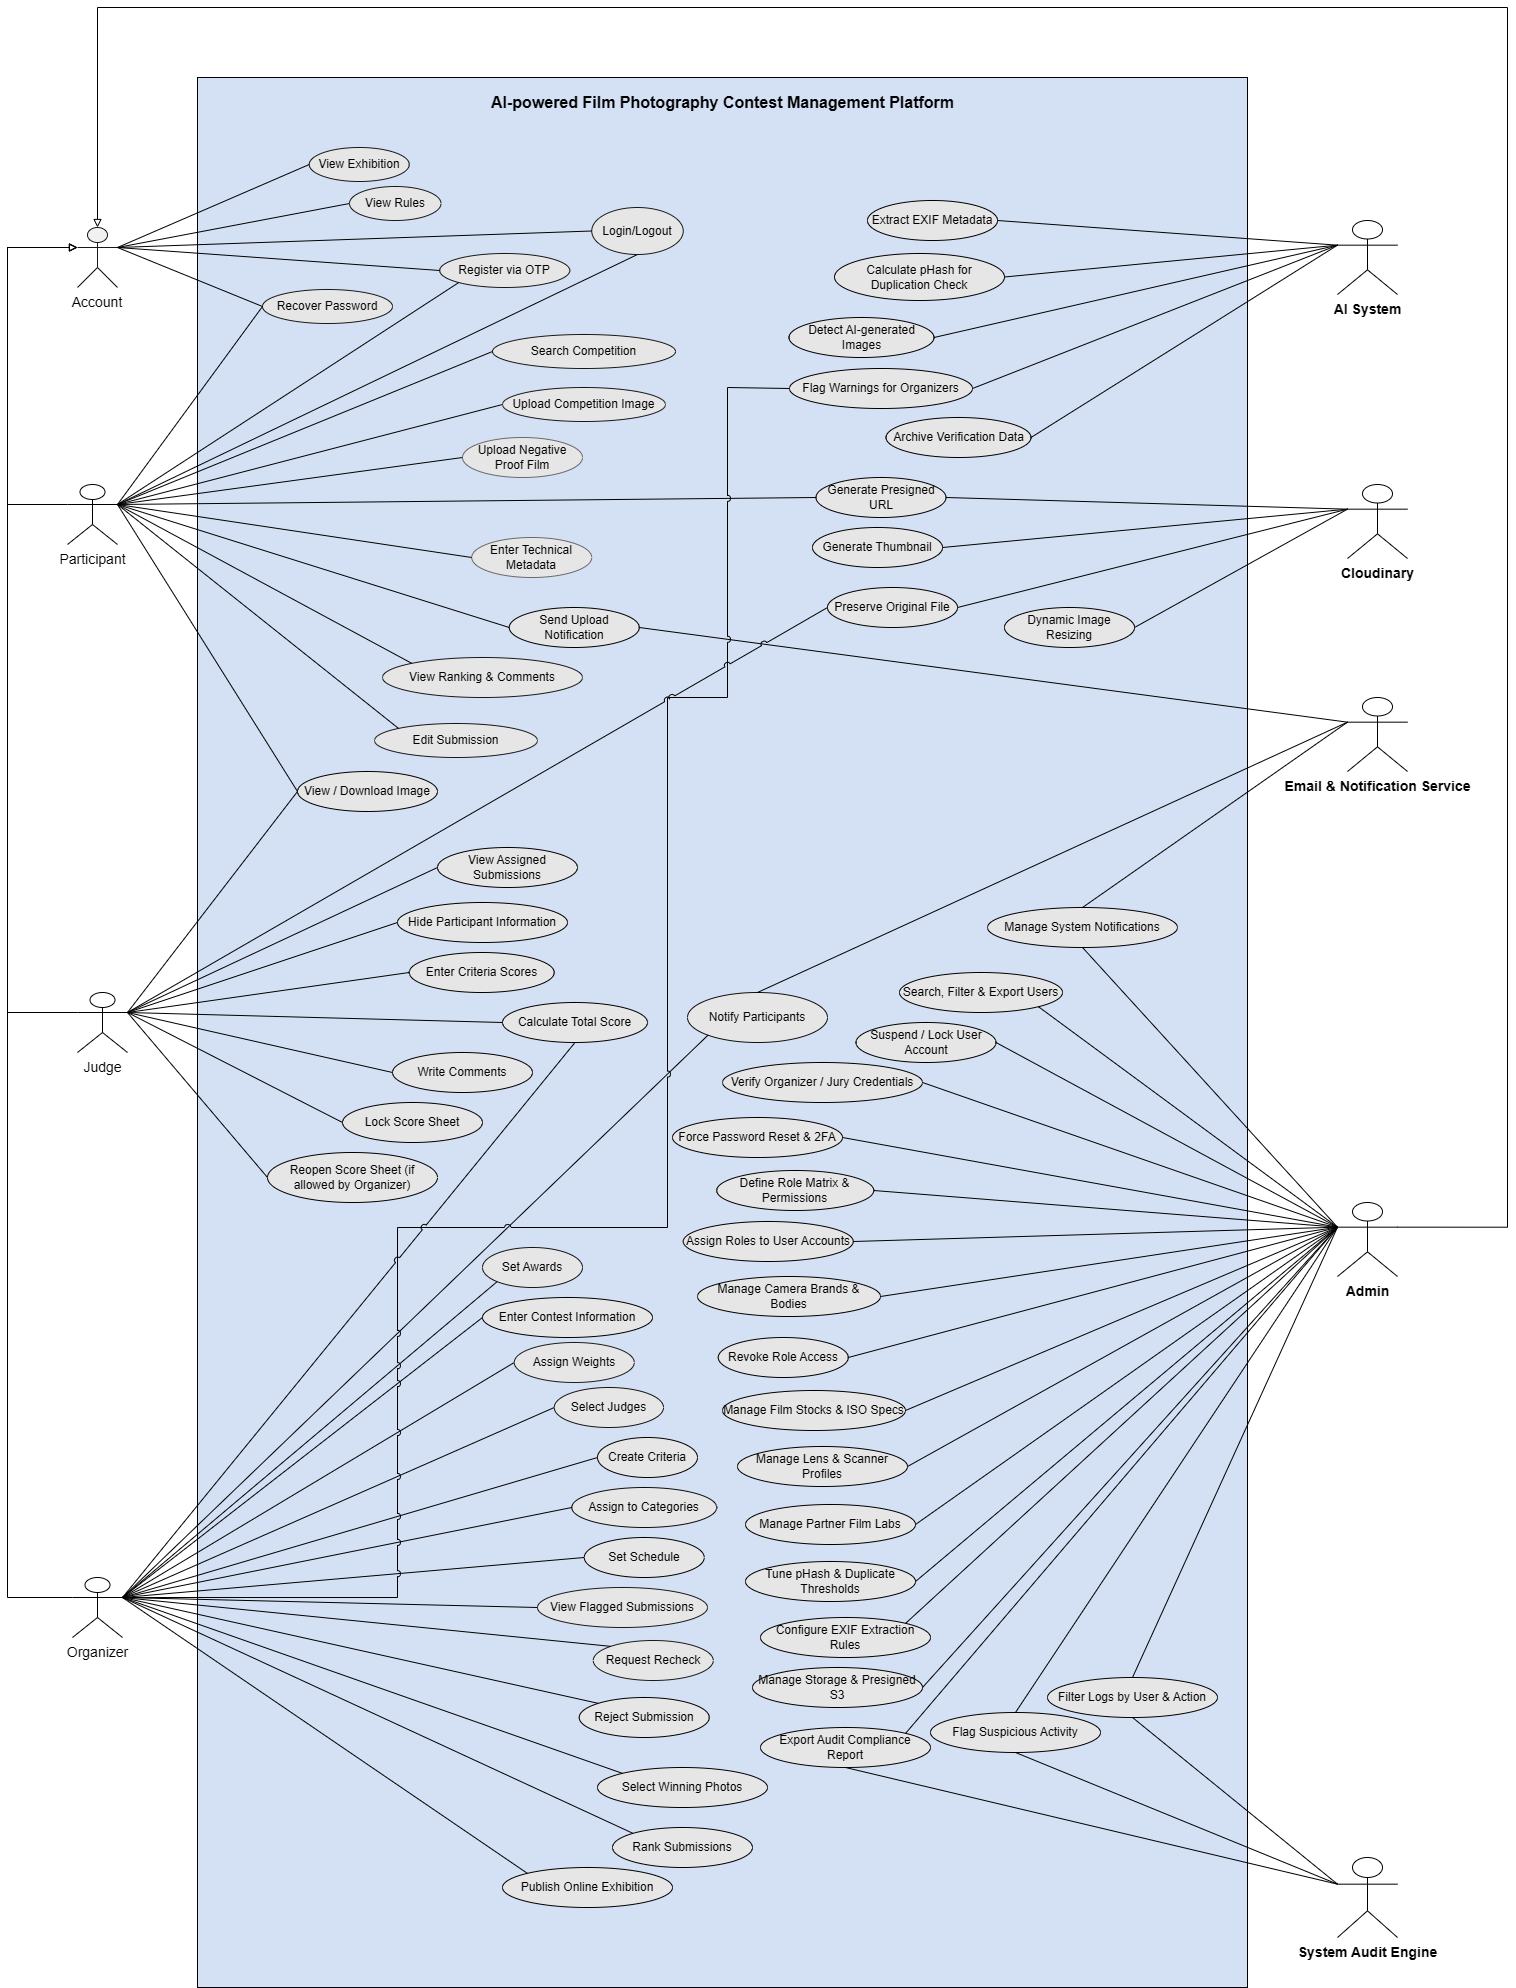
\includegraphics[width=0.95\textwidth]{images/use_case_diagram}
    \label{fig:use-case-diagram}
\end{figure}

\vspace{1em}
\paragraph*{2.2.2 Use Case Descriptions}
\label{par:use-case-descriptions}
\addcontentsline{toc}{paragraph}{\protect\numberline{2.2.2}Use Case Descriptions}

\vspace{0.5em}
\renewcommand{\arraystretch}{1.15}
\setlength{\tabcolsep}{4pt}
\small
\begin{longtable}{|>{\centering\arraybackslash}p{0.07\textwidth}|>{\raggedright\arraybackslash}p{0.20\textwidth}|>{\raggedright\arraybackslash}p{0.20\textwidth}|>{\raggedright\arraybackslash}p{0.45\textwidth}|}
\hline
\multicolumn{1}{|c|}{\textbf{ID}} & \multicolumn{1}{c|}{\textbf{Use Case}} & \multicolumn{1}{c|}{\textbf{Actors}} & \multicolumn{1}{c|}{\textbf{Use Case Description}} \\
\hline
UC-01 & View Exhibition & Account & Allows users to view the exhibition gallery displaying award-winning photo entries from past contests. \\
\hline
UC-02 & View Rules & Account & Displays the rules and regulations of a specific photography contest for users to review before participating. \\
\hline
UC-03 & Login/Logout & Account, Participant & Authenticates users via account credentials to grant access to the system, and allows secure session termination via Logout. \\
\hline
UC-04 & Register via OTP & Account, Participant & Allows users to register a new account using OTP (One-Time Password) verification sent to their email. \\
\hline
UC-05 & Recover Password & Account, Participant & Allows users to reset their forgotten password through email verification. \\
\hline
UC-06 & Search Competition & Participant & Allows participants to search and filter photography competitions by name, category, or status. \\
\hline
UC-07 & Upload Competition Images & Participant & Allows participants to upload their photo entries for a specific competition. \\
\hline
UC-08 & Upload Negative Proof Film & Participant & Allows participants to upload negative proof film images as evidence to verify the authenticity of their photo entries. \\
\hline
UC-09 & Enter Technical Metadata & Participant & Allows participants to input technical metadata for their submitted photo, such as camera, lens, ISO, aperture, and shutter speed. \\
\hline
UC-10 & Send Upload Notification & Participant, Email \& Notification Service & Automatically sends a notification to the participant's email confirming that their upload has been received. \\
\hline
UC-11 & Generate Presigned URL & Participant, Cloudinary & Generates a secure, time-limited URL that allows the participant's browser to upload images directly to Cloudinary storage. \\
\hline
UC-12 & View Ranking \& Comments & Participant & Allows participants to view their ranking results and comments left by judges for their submitted entries. \\
\hline
UC-13 & Edit Submission & Participant & Allows participants to edit the details of a previously submitted entry before the submission deadline. \\
\hline
UC-14 & View/Download Image & Participant, Judge & Allows participants and judges to view or download submitted images in their original quality for review or reference. \\
\hline
UC-15 & Preserve Original File & Judge, Cloudinary & Ensures that the original uploaded image is securely stored in Cloudinary without modification, allowing judges to access the original file whenever needed. \\
\hline
UC-16 & View Assigned Submissions & Judge & Allows the Judge to view the list of submissions assigned to them by the Organizer for a given contest category or judging round, including entry thumbnail, ID, and technical metadata, before starting evaluation. \\
\hline
UC-17 & Hide Participant Information & Judge & Enables blind (anonymous) judging by hiding the submitting participant's identifying information (name, account, portfolio link) from the Judge's view during scoring, ensuring an unbiased evaluation. \\
\hline
UC-18 & Enter Criteria Scores & Judge & Allows the Judge to input a numerical score for each submission against every evaluation criterion (e.g., creativity, composition, technical execution, film grain) defined by the Organizer for that contest. \\
\hline
UC-19 & Calculate Total Score & Judge, Organizer & Automatically computes the weighted total score for each submission by combining the individual criterion scores entered by the Judge with the weight assigned to each criterion, used by the Organizer to determine rankings. \\
\hline
UC-20 & Write Comments & Judge & Allows the Judge to add a qualitative critique or feedback text for a submission alongside its numeric score, providing context for the participant and the Organizer. \\
\hline
UC-21 & Lock Score Sheet & Judge & Allows the Judge to lock their score sheet for a submission once evaluation is complete, preventing further edits and confirming the score as final. \\
\hline
UC-22 & Reopen Score Sheet & Judge, Organizer & Allows the Organizer to unlock a previously locked score sheet (e.g., on the Judge's request or in case of an error/dispute), enabling the Judge to revise scores or comments before results are finalized. \\
\hline
UC-23 & Flag Warmings for Organizers & Organizer, AI System & The AI System automatically flags a submission with a warning — such as a duplicate (pHash) match, suspected AI-generated content, or EXIF inconsistency — and sends the flag report to the Organizer for manual review. \\
\hline
UC-24 & Notify Participants & Organizer, Email \& Notification Service & Allows the Organizer to trigger notifications (email/push) to participants regarding contest updates, submission status, dispute outcomes, or final results, delivered through the Notification Service. \\
\hline
UC-25 & Set Awards & Organizer & Allows the Organizer to define the award structure for a contest, including award categories, number of winners per category, and prize details. \\
\hline
UC-26 & Enter Contest Information & Organizer & Allows the Organizer to create and configure a new contest by entering its name, theme, categories, timeline, and rules. \\
\hline
UC-27 & Assign Weights & Organizer & Allows the Organizer to configure the weight (percentage contribution) of each judging criterion used when calculating a submission's total score. \\
\hline
UC-28 & Select Judges & Organizer & Allows the Organizer to select and assign Judges to a contest or specific category, including allocating them to particular judging rounds. \\
\hline
UC-29 & Create Criteria & Organizer & Allows the Organizer to define and manage the set of scoring criteria (e.g., creativity, storytelling, technical execution) that Judges will use to evaluate submissions in a contest. \\
\hline
UC-30 & Assign to Categories & Organizer & Allows the Organizer to classify and assign submitted photographs to their appropriate contest categories or divisions for organized judging and ranking. \\
\hline
UC-31 & Set Schedule & Organizer & Allows the Organizer to configure the contest timeline, including submission period, judging period, recheck deadline, and winner announcement schedule. \\
\hline
UC-32 & View Fagged Submissions & Organizer & Displays the list of submissions flagged by the AI verification system for duplicate detection, AI-generated content, or metadata inconsistencies, allowing the Organizer to review them. \\
\hline
UC-33 & Request Recheck & Organizer & Enables the Organizer to request an additional review for a submission when suspicious content or scoring discrepancies are identified. \\
\hline
UC-34 & Reject Submission & Organizer & Allows the Organizer to reject submissions that violate contest regulations, fail verification, or do not meet eligibility requirements. \\
\hline
UC-35 & Select Winning Photos & Organizer & Enables the Organizer to select winning submissions based on judges' scores, contest rules, and verification results before publication. \\
\hline
UC-36 & Rank Submissions & Organizer & Automatically or manually ranks submissions according to judges' scores and predefined contest criteria to determine final standings. \\
\hline
UC-37 & Publish Online Exhibition & Organizer & Allows the Organizer to publish approved winning photos to the online exhibition, making them available for public viewing. \\
\hline
UC-38 & Extract EXIF Metadata & AI System & Automatically extracts EXIF metadata from uploaded images to verify camera information, capture settings, and image authenticity. \\
\hline
UC-39 & Calculate pHash for Duplication Check & AI System & Generates perceptual hash (pHash) values to compare uploaded images and identify duplicate or highly similar submissions. \\
\hline
UC-40 & Detect AI-generated Images & AI System & Analyzes uploaded images using AI detection techniques to identify whether the image was generated or manipulated by artificial intelligence. \\
\hline
UC-41 & Archive Vertification Data & AI System & Stores verification results, extracted metadata, and AI analysis records for auditing, dispute resolution, and future reference. \\
\hline
UC-42 & Generate Thumbnail & Cloudinary & Automatically generates optimized thumbnail versions of uploaded images for previews, galleries, and faster loading. \\
\hline
UC-43 & Dynamic Image Resizing & Cloudinary & Dynamically resizes images into different resolutions while preserving image quality for various display devices. \\
\hline
UC-44 & Manage System Notifications & Admin, Email \& Notification Service & Allows the Admin to configure notification templates and events, while the Email Notification Service delivers OTPs, status updates, and contest notifications to users. \\
\hline
UC-45 & Search, Filter \& Export Users & Admin & Enables the Admin to search, filter, and export user information for administration, reporting, and system management purposes. \\
\hline
UC-46 & Suspend/Lock User Account & Admin & Allows the Admin to temporarily suspend or permanently lock user accounts upon detecting policy violations. \\
\hline
UC-47 & Verify Organizer/Jury Credentials & Admin & Allows the Admin to verify profiles and approve the identities and credentials of Organizers or Jury members. \\
\hline
UC-48 & Force Password Reset \& 2FA & Admin & Allows the Admin to force users to reset their passwords and set up Two-Factor Authentication (2FA) upon their next login. \\
\hline
UC-49 & Define Role Matrix \& Permissions & Admin & Allows the Admin to configure the role-based access control (RBAC) matrix, specifying detailed permissions for each system role. \\
\hline
UC-50 & Assign Roles to User Accounts & Admin & Allows the Admin to assign specific roles and privileges to individual user accounts within the system. \\
\hline
UC-51 & Manage Camera Brands \& Bodies & Admin & Allows the Admin to add, update, or delete categories of analog camera brands and camera bodies. \\
\hline
UC-52 & Revoke Role Access & Admin & Allows the Admin to partially or fully revoke access permissions previously granted to a user account. \\
\hline
UC-53 & Manage Film Stocks \& ISO Specs & Admin & Allows the Admin to manage the catalog of film stocks and their corresponding ISO specifications. \\
\hline
UC-54 & Manage Lens \& Scanner Profiles & Admin & Allows the Admin to manage configurations and metadata profiles for various camera lenses and film scanners. \\
\hline
UC-55 & Manage Partner Film Labs & Admin & Allows the Admin to add, update, or remove information regarding partner film processing labs. \\
\hline
UC-56 & Tune pHash \& Duplicate Thresholds & Admin & Allows the Admin to adjust the pHash algorithm and similarity thresholds to optimize the detection of duplicate or plagiarized images. \\
\hline
UC-57 & Configure EXIF Extraction Rules & Admin & Allows the Admin to define rules for parsing and extracting EXIF metadata from uploaded images. \\
\hline
UC-58 & Manage Storage \& Presigned S3 & Admin & Allows the Admin to manage storage capacity and configure secure upload links (Presigned URLs) via Amazon S3. \\
\hline
UC-59 & Export Audit Compliance Report & Admin, System Audit Engine & Allows the generation and exporting of audit reports regarding system security compliance and data integrity. \\
\hline
UC-60 & Flag Suspicious Activity & Admin, System Audit Engine & The system automatically flags suspicious activities (e.g., spam, hacking attempts) and alerts the Admin for resolution. \\
\hline
UC-61 & Filter Logs by User & Admin, System Audit Engine & Allows the Admin to search, filter, and view detailed system activity logs for specific user accounts. \\
\hline
\end{longtable}